\documentclass{beamer}

\usepackage{graphicx}

\usetheme[subsectionpage=progressbar]{metropolis}           % Use metropolis theme
\definecolor{Blue}{HTML}{306D9F}
\definecolor{Orange}{HTML}{CF4A30}

% Theme colors are derived from these two elements
\setbeamercolor{alerted text}{fg=Orange}


\setbeamercolor{normal text}{fg=Blue}
% ... however you can of course override styles of all elements
\setbeamercolor{frametitle}{bg=Blue}

\title{
    \centering
    {
\includegraphics[width=0.75\textwidth]{res/logo}}
}

\date{
    \today
}

\author{
    Alberto Amigo Alonso \\
    Sergio Delgado Álvarez \\
    Sergio García Prado \\
    Oscar Fernández Angulo \\
    Silvia Rodriguez Ares \\
}

\institute{Universidad de Valladolid}

\begin{document}
    \maketitle

    \section{El servicio}

        \subsection{¿Qué es?}

            \begin{frame}{¿Qué es?}
                Servicio web destinado a permitir a remitentes y destinatarios ofertar envíos para que los transportistas sean capaces de encontrarlos permitiendo a todos los usuarios monitorizarlos
            \end{frame}

        \subsection{¿Cómo funciona?}
            \begin{frame}{¿Cómo funciona?}
                \begin{itemize}
                    \item Los clientes del servicio (remitentes y transportistas) ofertan envíos.

                    \item Los transportistas buscan estos envíos y además pujan un precio por el cual están dispuestos a llevar a cabo el servicio.
                \end{itemize}
            \end{frame}

            \begin{frame}{¿Cómo funciona?}
                \begin{itemize}
                    \item Después los clientes seleccionan al transportista que mejor les convenga acorde a sus necesidades.

                    \item Durante todo el proceso de envío ambas partes interactuan entre sí para conseguir un mayor grado de satisfacción entre ambos.
                \end{itemize}
            \end{frame}

            \begin{frame}{¿Cómo funciona?}
                \begin{itemize}
                    \item Una vez finalizado el envío ambas partes se pueden valorar.

                    \item Estas métricas serán las que en posteriores envíos utilizarán el resto de usuarios.
                \end{itemize}
            \end{frame}

    \section{Implementación}

        \subsection{Introducción}

            \begin{frame}{Tecnologías Utilizadas}
                \begin{itemize}
                    \item FrontEnd
                    \begin{itemize}
                        \item Angular.js
                        \item Bootstrap
                    \end{itemize}

                    \item BackEnd
                    \begin{itemize}
                        \item Java J2EE
                        \begin{itemize}
                            \item Jersey
                            \item Java JWT
                            \item Apache Derby
                        \end{itemize}
                    \end{itemize}
                \end{itemize}

                \begin{figure}
                    \centering
                    \begin{minipage}{0.32\textwidth}
                        
\includegraphics[width=\textwidth]{res/logo-jersey}
                    \end{minipage}
                    \begin{minipage}{0.32\textwidth}
                        
\includegraphics[width=\textwidth]{res/logo-angular}
                    \end{minipage}
                    \begin{minipage}{0.32\textwidth}
                        
\includegraphics[width=\textwidth]{res/logo-bootstrap}
                    \end{minipage}
                \end{figure}
            \end{frame}

            \begin{frame}{Modelo Rest}
                \begin{figure}
                    \centering
                    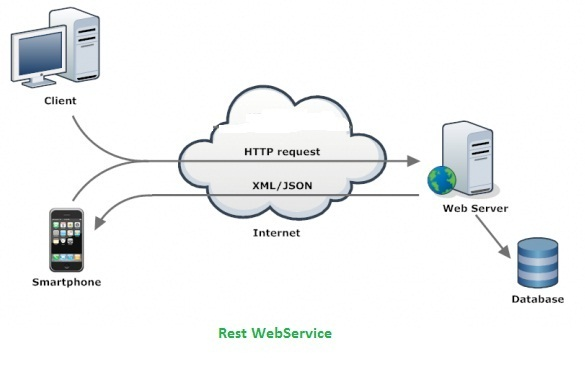
\includegraphics[width=\textwidth]{res/rest-webservices}
                \end{figure}
            \end{frame}

        \subsection{FrontEnd}

            \begin{frame}{FrontEnd}

            \end{frame}

            \begin{frame}{Angular.js}

            \end{frame}

            \begin{frame}{Bootstrap}

            \end{frame}

        \subsection{BackEnd}

            \begin{frame}{BackEnd}

            \end{frame}

            \begin{frame}{Jersey}

            \end{frame}

            \begin{frame}{Java JWT}

            \end{frame}

            \begin{frame}{Apache Derby}

            \end{frame}
    \begin{frame}[standout]
        ¿Preguntas?
    \end{frame}

\end{document}
